移动之后,已移动的对象既没有部分销毁,也没有完全销毁。析构函数还未调用,直到已移动对象的生命周期结束时才调用。因此,析构函数至少要没问题。\par

然而,C++标准库为可移动类型提供了更多的保证。已移动对象处于“有效但未定义的状态”,所以可以像使用任何不知道其值的类型的对象一样使用已移动对象。像使用该类型的非\textit{const}引用形参,而不知道所传递对象的值一样。例如,可以做的不仅仅是销毁已移动对象,还可以使用移动语义来实现排序和可变序列算法。\par

为了更详细地理解如何处理已移动对象,最好区分与之相关的信息:\par

\begin{itemize}
	\item C++标准库安全地使用已移动对象有什么要求?
	\item 给已移动对象什么样的保证,才能让这些类型的用户知道如何使用?
\end{itemize}

至少应该满足C++标准库的要求。\par

\hspace*{\fill} \par %插入空行
\textbf{6.1.1 已移动对象的状态要求}

C++标准库对已移动对象的要求没有什么特别的。对于任何函数,为传递的类型和对象制定的需求,也适用于任何内部传递或是移动来的对象。\par

已移动对象必须能够销毁。此外,必须能够将新值赋给已移动对象。\par

例如,考虑如何交换两个对象\textit{a}和\textit{b}(这可能是排序操作的一部分)。交换的实现通常如下(见图6.1):\par

\begin{itemize}
	\item 将\textit{a}移动到一个新的临时对象\textit{tmp}(这样\textit{a}就变成了已移动的对象)。
	\item 将\textit{b}移动赋值给\textit{a}(这样\textit{b}就成为了已移动对象)。
	\item 将\textit{tmp}移动赋值给\textit{b}(这样\textit{tmp}就成了已移动对象)。
	\item 销毁已移动对象\textit{tmp}。
\end{itemize}

\begin{center}
	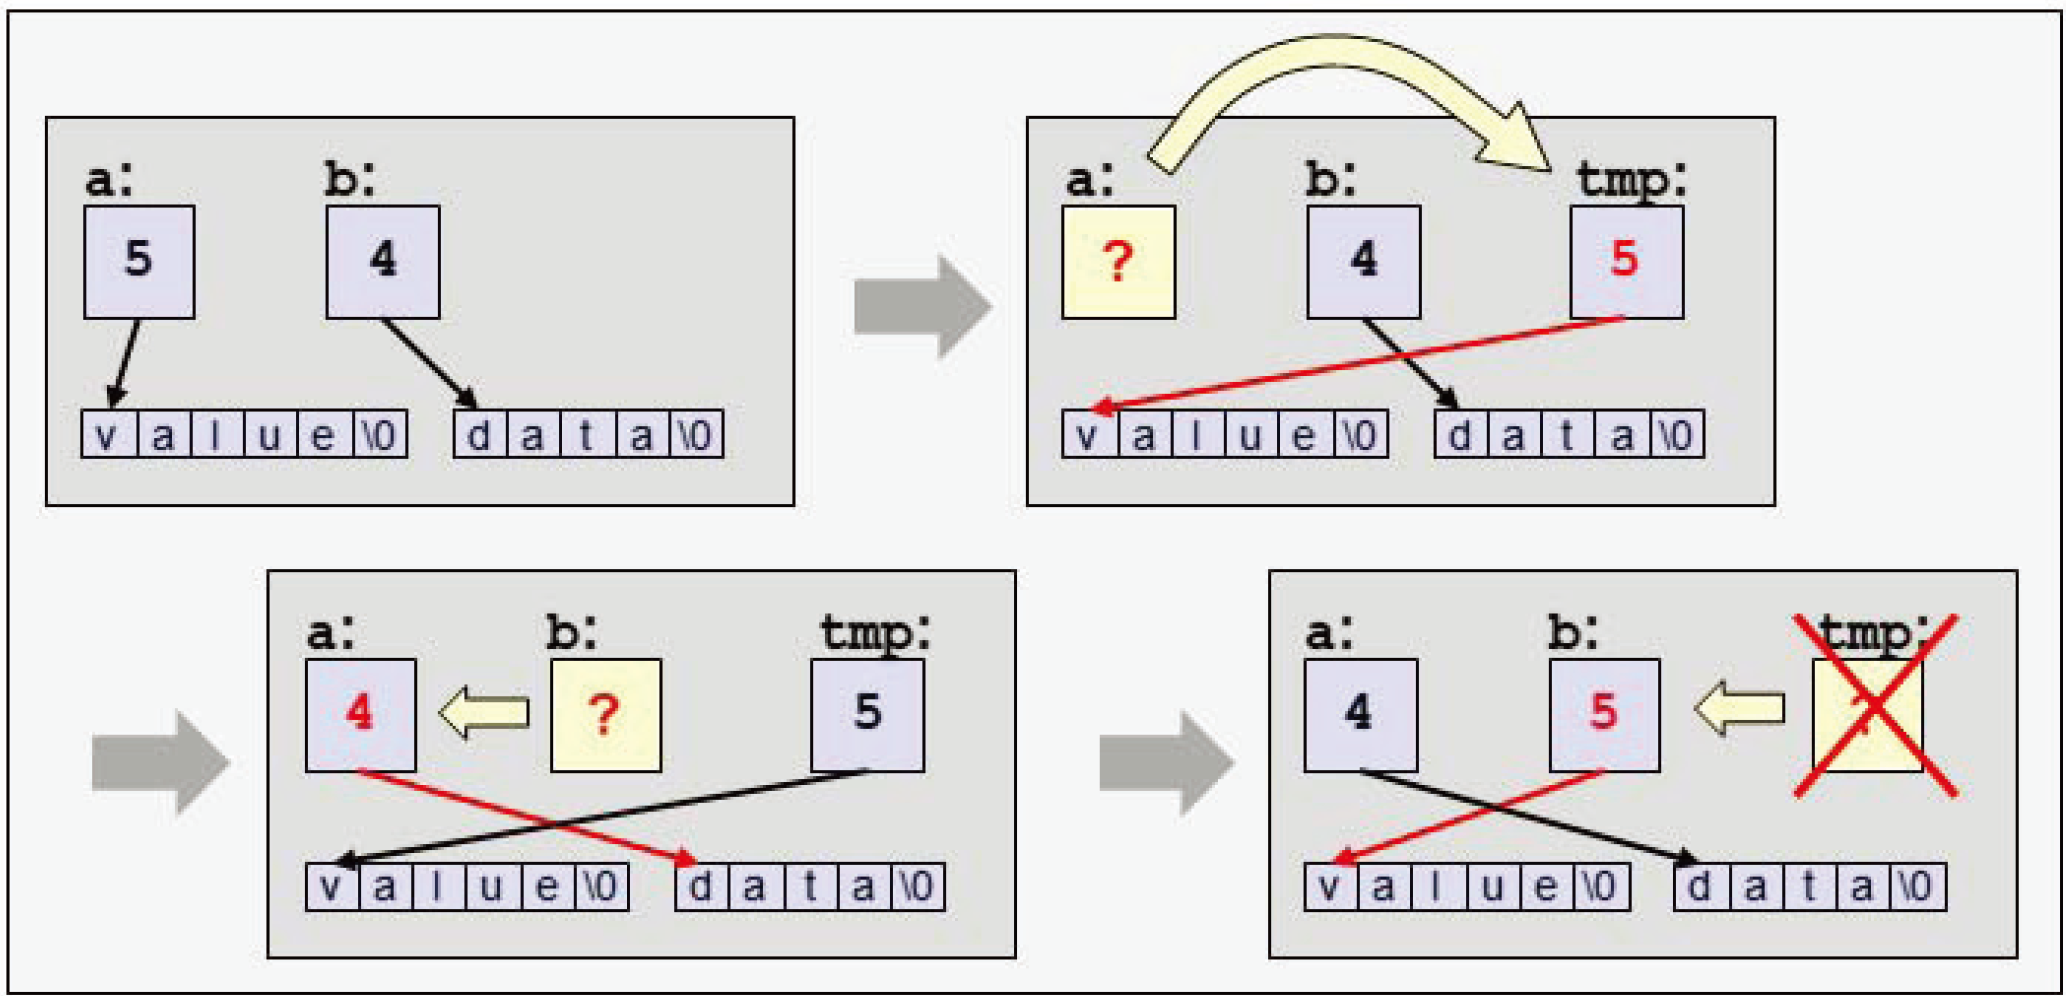
\includegraphics[width=1.0\textwidth]{content/1/chapter6/images/1}
\end{center}

注意,可以通过向两个参数传递相同的对象来实现自交换。这种情况下,可以将状态为已移动的对象赋值给它自己。\par

所以,对于已移动对象,有同样的要求,适用于所有对象:\par

\begin{itemize}
	\item 必须能够销毁已移动对象。
	\item 必须能够为已移动对象赋值。
	\item 应该能够复制、移动或将已移动对象赋值给另一个对象。
\end{itemize}

已移动对象还能够处理特殊操作的额外需求。例如排序,所以必须支持<操作符,或有相应的排序标准,这也适用于已移动的对象。您可能会争辩说,排序算法中应该知道哪个对象移动了,这样就可以避免比较它,但C++标准库并不要求这样做。顺便一说,您可以传递已移动对象,对它们进行排序,只要支持所有必需的操作就可以了。\par

注意,C++标准库的定义需要的不仅仅是Alexander Stepanov和Paul McJones在《编程元素》一书的内容。\par

对于C++标准库中使用的所有对象和类型,应该确保已移动对象也支持所调用函数的要求。\par

\hspace*{\fill} \par %插入空行
\textbf{6.1.2 保证已移动对象的状态}

已移动对象的保证定义在使用哪些代码。通常,类的设计者决定给出哪些保证,并且总在生命周期结束时销毁对象。对于移动状态,必须提定义良好的析构函数。\par

通常,会有更多要保障的。对于C++标准库的要求,支持基本操作,如复制、赋值相同类型的对象通常就足够了。然而,用户通常希望可以使用处理所有其他方式来为对象赋值。因此,保证可以将新值“赋值”给已移动对象就非常有用。\par

考虑给标准字符串\textit{s}赋新值的不同方法:\par

\begin{lstlisting}[caption={}]
s = "hello"; // assign ”hello”
s.assign(s2); // assign the state of s2
s.clear(); // assign the empty state
std::cin >> s; // assign the next word from standard input
std::getline(myfile, s); // assign the next line from a file
\end{lstlisting}

例如,下面的循环是将流逐行读入vector对象的常用方法:\par

\begin{lstlisting}[caption={}]
std::string row;
while (std::getline(myStream, row)) {
	coll.push_back(std::move(row)); // move the line into the vector
}
\end{lstlisting}

另一个例子中,可以在处理容器的泛型代码中实现以下语句:\par

\begin{lstlisting}[caption={}]
foo(std::move(obj)); // pass obj to foo()
obj.clear(); // ensure the object is empty afterwards
\end{lstlisting}

类似的代码可以用于释放指针所使用的对象的内存:\par

\begin{lstlisting}[caption={}]
draw(std::move(up)); // the unique pointer might or might not give up ownership
up.reset(); // ensure we give up ownership and release any resource
\end{lstlisting}

通过声明,已移动对象处于有效但未定义的状态,C++标准为其库中的操作进行了保证。\par

例如,以下是根据C++标准定义的行为:\par

\begin{lstlisting}[caption={}]
std::stack<int> stk;
...
foo(std::move(stk)); // stk gets unspecified state
stk.push(42);
... // do something else without using stk
int i = stk.top();
assert(i == 42); // should never fail
\end{lstlisting}

虽然不知道通过\textit{std::move()}将\textit{stk}传递给\textit{foo()}后的值,但只要使用它来保存\textit{42},直到再次需要,都可以将它当做有效的堆栈。\par

当然,所提供的保证能达到什么程度取决于您,但要确保您的类型的用户知道这些保证。通常,希望您的类型提供与C++库相同的保证,这样就可以像使用该类型的任何其他对象一样使用已移动对象了。\par

\hspace*{\fill} \par %插入空行
\textbf{6.1.3 破坏不变量}

C++标准库定义了所有处于“有效但未定义状态”的移动对象的含义如下:\par

\textit{对象的值没有指定,除非满足对象的不变量,并且对象上的操作按照指定的类型进行}\par

\hspace*{\fill} \par %插入空行
不变量是适用于所有对象。有了这个保证,可以假定已移动的对象处于某种状态,这意味着它的不变量没有破坏。可以像使用非\textit{const}引用参数一样使用对象,而不知道传递的参数的任何信息:可以调用任何没有约束或前置条件的操作,并且效果/结果是为该类型的其他对象指定。\par

例如,对于已移动的字符串,可以执行没有先决条件的操作:\par

\begin{itemize}
	\item 查询大小
	\item 打印输出
	\item 遍历字符
	\item 转换为C字符串
	\item 分配新值
	\item 添加字符
\end{itemize}

此外,所有这些函数具有语义:\par

\begin{itemize}
	\item 返回的大小可以安全地调用索引操作符。
	\item 返回的大小与迭代时的字符数相匹配。
	\item 遍历字符时,打印的字符与字符序列匹配。
	\item 添加一个字符将把该字符放在值的末尾(不知道是否还有其他字符在前面)。
\end{itemize}

开发者可以利用这些保证(参见std::stack<>的例子)。\par

有时候,必须确保不破坏不变量,否则默认的特殊移动成员函数无法正常工作。在下面的小节中根据示例进行讨论。\par

\hspace*{\fill} \par %插入空行
\textbf{受限的不变量}

不把C++标准库的全部保证给已移动状态的对象也可以。也就是说,可能有意地限制已移动对象的操作。例如,当对象的有效状态总是需要诸如内存之类的资源时,只有一个部分支持的状态可能会更好地降低移动操作的成本。\par

理想情况下,不支持所有操作的状态是可查的。对象应该知道这个状态,并提供成员函数来检查这个状态。已移动对象也可能拒绝执行此状态下不支持的操作。然而,相应的检查可能会影响性能。\par

C++标准库中,有些类型提供了API来检查对象是否处于移出状态。例如,std::futures有一个成员函数valid(),该函数对已移动对象返回false。所以,不同对象检查状态(是否移动)的接口不同。\par

通常,已移动状态是默认构造状态,这意味着已移动状态是不变量的一部分。任何情况下,需要让用户知道什么是可用的,什么不可用。\par




